\chapter{Общие уравнения симметрично-противоточного каскада}


\section{Понятие разделительного элемента, ступени, каскада.}


\subsection{Понятие разделительного элемента}

В общем случае разделительный элемент может иметь несколько входов и выходов. В практике разделения изотопов однофазными методами, он имеет, как правило, один вход и два выхода и называется \textit{простым разделительным элементом} (рис. \ref{1_1}). В этом случае в разделительный элемент подают поток разделяемой смеси $L_\textup{э}$ с концентрацией (мольной долей, так как если речь идет о разделении изотопов тяжелых элементов, то в этом случае величины мольной и массовой концентрации практически совпадают) ценного (целевого изотопа) $c$, а из него отбирают два потока: «обогащенный», с более высокой, чем во входящем потоке, концентрацией $c'$, и «обедненный», с более низкой концентрацией $c''$. В отсутствие потерь рабочего вещества, которые могут быть вызваны, например, его частичным разложением в процессе разделения, обогащенный поток будет равен $L'_\textup{э} =\theta L_\textup{э} $, а обедненный, соответственно,~~$L''_\textup{э} =(1-\theta )L_\textup{э}$. Отношение $\theta =\frac{L'_\textup{э}}{L_\textup{э}} $ называют \textit{коэффициентом деления потока}, а расход $L_\textup{э}$ -- \textit{производительностью элемента}. 


\begin{figure}[ht]
  \centerfloat{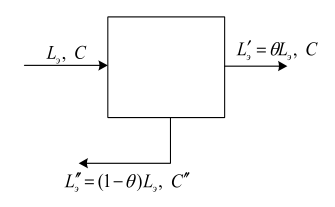
\includegraphics[scale=0.9]{img/sep_el.png}}
  \caption{Схема разделительной ступени }\label{1_1}
\end{figure}


\subsection{Понятие разделительной ступени}


В разделительную ступень параллельно соединяют элементы с одинаковыми величинами $\theta $, $c,$ $ $$c'$ и $c''$ (рис. \ref{1_1}). Она имеет суммарную производительность $L$ и выходящие потоки $L'_{} =\theta L_{}$ и $L''_{} =(1-\theta )L_{}$. Такое представление о работе элементов в ступени предполагает, что все они работают в одинаковых условиях и имеют одинаковые характеристики.

Между приращением $\delta '=c'-c$ и уменьшением $\delta ''=c-c''$ концентрации целевого компонента в выходящих потоках разделительного элемента существует определенная связь. Для стационарного состояния эта связь может быть найдена из следующих уравнений материального баланса:

\begin{equation} \label{GrindEQ__1_1_} 
L=L'+L'', 
\end{equation} 

\begin{equation} \label{GrindEQ__1_2_} 
Lc=L'(c+\delta ')+L''(c-\delta ''). 
\end{equation} 

Из \ref{GrindEQ__1_1_} и \ref{GrindEQ__1_2_} следует, что 

\begin{equation} \label{GrindEQ__1_3_} 
\delta ''=\frac{L'}{L''} \delta '=\frac{\theta }{1-\theta } \delta '. 
\end{equation} 

Одной из основных разделительных характеристик ступени является \textit{полный коэффициент разделения}, который для большинства однофазных методов разделения не зависит от состава изотопной смеси
\begin{equation} \label{GrindEQ__1_4_} 
q={\frac{c'}{1-c'}  \mathord{\left/{\vphantom{\frac{c'}{1-c'}  \frac{c''}{1-c''} =\frac{R'}{R''} }}\right.\kern-\nulldelimiterspace} \frac{c''}{1-c''} =\frac{R'}{R''} } .                              
\end{equation} 

Здесь $R'$ и $R''$ - значения относительной концентрации ценного (целевого) изотопа ($R=\frac{c}{1-c} $) в потоках обогащенной и обедненной фракции. Коэффициент разделения $q$ характеризует эффект разделения, достигаемый в одном элементе или ступени, и может зависеть от производительности ступени $L$ и коэффициента деления потока $\theta $:

\begin{equation} \label{GrindEQ__1_5_} 
q=q(L,\theta ), 
\end{equation} 

где $q(L,\theta )$ - некоторая функция, которую определяют по результатам теоретических или экспериментальных исследований.

В соответствии со сказанным к числу основных параметров ступени относятся восемь величин: $L,\; L',\; L'',\; c,\; c',\; c'',\; q,\; \theta $, связанных независимыми соотношениями \ref{GrindEQ__1_1_}~--\ref{GrindEQ__1_5_}. Причём из перечисленных параметров свободными (независимыми) являются только три. Как правило, в качестве свободных параметров рассматривают величины $L,\; \; c\; $ и $\theta $. Однако, в зависимости от рассматриваемой задачи могут быть выбраны их различные комбинации.

Для удобства анализа эффекта разделения в элементе (ступени) могут быть введены дополнительные параметры и характеристики. Например, коэффициенты разделения по обогащённой $\alpha $ и обеднённой $\beta $ фракциям, рассчитываемые как

\begin{equation} \label{GrindEQ__1_6_} 
\alpha ={\frac{c'}{1-c'}  \mathord{\left/{\vphantom{\frac{c'}{1-c'}  \frac{c}{1-c} }}\right.\kern-\nulldelimiterspace} \frac{c}{1-c} }  , \beta ={\frac{c}{1-c}  \mathord{\left/{\vphantom{\frac{c}{1-c}  \frac{c''}{1-c''} }}\right.\kern-\nulldelimiterspace} \frac{c''}{1-c''} } .        
\end{equation} 

Эти параметры характеризуют величину эффекта разделения в обогащённой и обеднённой фракции по отношению к концентрации в потоке питания. Кроме того, для описания процесса разделения удобно пользоваться коэффициентами обогащения $\varepsilon $, $\varepsilon '$, $\varepsilon ''$, равными

\begin{equation} \label{GrindEQ__1_7_} 
\varepsilon =q-1, \varepsilon '=\alpha -1, \varepsilon ''=1-{1 \mathord{\left/{\vphantom{1 \beta }}\right.\kern-\nulldelimiterspace} \beta } .             
\end{equation} 

Набор параметров $\varepsilon $, $\varepsilon '$, $\varepsilon ''$ позволяет определить \textit{полное обогащение ступени}
\begin{equation} \label{GrindEQ__1_8_} 
\delta =c'-c''=\delta '+\delta '',                          
\end{equation} 

где $\delta '=c'-c$, $\delta ''=c-c''$. Если выразить $c'$ и $c''$ из \ref{GrindEQ__1_6_} и использовать \ref{GrindEQ__1_7_}, то в результате получим
\begin{equation} \label{GrindEQ__1_9_} 
\delta '=\frac{\varepsilon 'c(1-c)}{1+\varepsilon 'c}  ,  \delta ''=\frac{\varepsilon ''c(1-c)}{1-\varepsilon ''c} .              
\end{equation} 

Отсюда видно, что при заданных коэффициентах $\varepsilon '$, $\varepsilon ''$ зависимости $\delta '$ и $\delta ''$ от $c$ имеют максимумы, не совпадающие друг с другом. В случае «слабого обогащения» ($\varepsilon =q-1<<1$) наибольшие значения $\delta '$ и $\delta ''$ достигаются в одной точке $c=0,5$, а формулы \ref{GrindEQ__1_9_} существенно упрощаются:

\begin{equation} \label{GrindEQ__1_10_} 
\delta '=\varepsilon 'c(1-c),  \delta ''=\varepsilon ''c(1-c).              
\end{equation} 

При подстановке \ref{GrindEQ__1_10_} в \ref{GrindEQ__1_8_} имеем

\begin{equation} \label{GrindEQ__1_11_} 
\delta =\varepsilon c(1-c),  \varepsilon '=\varepsilon (1-\theta ), \varepsilon ''=\theta \varepsilon .    
\end{equation} 

Согласно \ref{GrindEQ__1_3_} и \ref{GrindEQ__1_8_} обогащения $\delta $, $\delta '$, $\delta ''$ связаны друг с другом балансовыми соотношениями

\begin{equation} \label{GrindEQ__1_12_} 
\delta '=(1-\theta )\delta ,  \delta ''=\theta \delta .                             
\end{equation} 

Следовательно, если коэффициенты разделения не зависят от параметров $L$ и $\theta $, можно путем уменьшения $\theta $ повысить концентрацию ценного компонента в обогащённом потоке $c'$, произведя таким образом «перераспределение» полного обогащения $\delta $ в выходных потоках. При этом концентрация в обеднённом потоке $c''$ будет приближаться к концентрации во входном потоке $A$. Очевидно, что возможность такого изменения обогащений $\delta '$ и $\delta ''$ связана с условиями сохранения материального баланса в разделительном элементе.

\subsection{Понятие каскада.}


Для получения требуемых концентраций ценного (целевого) изотопа ступени соединяют в последовательную цепочку -- каскад, умножающий эффект разделения в одиночной разделительной ступени. Простейшей схемой последовательного соединения ступеней является так называемый \textit{простой каскад} (рис. \cite{cas}). Его отличительным признаком является подача обогащенной фракции на питание следующей ступени и выведение потоков обедненной фракции ступеней из процесса дальнейшей переработки. В такой схеме поток питания каскада \textit{F} (от английского слова Feed) подают в первую ступень, поток отбора \textit{P} (Product) является потоком обогащенной фракции последней n-ой ступени. Отвальный поток каскада \textit{W} (Waste) образуют обедненные потоки ступеней (могут не смешиваться друг с другом). Так как эти потоки не участвуют в процессе обогащения, то простой каскад, по существу, является прямоточным. Для разделения изотопов, когда разделяемое вещество, как правило, является дорогим, простой каскад является неэффективным. Это обусловлено существенным сокращением потоков питания ступеней и выведением в отвал потоков с концентрацией ценного (целевого) изотопа, близкой к концентрации в обогащенных фракциях. Поэтому при разделении изотопов применяют более эффективную с точки зрения экономии сырья, а также  имеющую ряд других преимуществ, противоточную (рециркуляционную) схему, в которой обедненная ценным компонентом фракция возвращается в каскад для дальнейшей переработки. Простейшая схема такого каскада приведена на рис. \cite{image2}. В этой схеме обогащенный поток $L'_{s} =\theta _{s} L_{s} $ из произвольной $s$-ой ступени подается на вход последующей $s+1$-ой ступени, а обедненный $L''_{s} =(1-\theta _{s} )L_{s} $-- на вход $s-1$-ой ступени. При таком соединении на входе в $s$-ую ступень смешиваются потоки из предыдущей $s-1$-ой ступени и из последующей $s+1$-ой. Такой каскад является \textit{противоточным}, а способ соединения ступеней с помощью внешних коммуникаций, т.е. таких коммуникаций, в которых передаются уже разделенные потоки, называют\textit{ внешним каскадированием}.

\begin{figure}[ht]
  \centerfloat{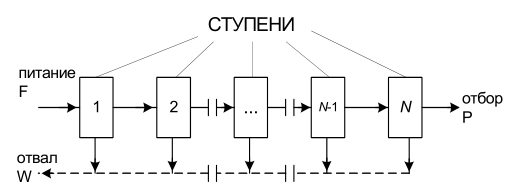
\includegraphics[scale=0.9]{img/cas.png}}
  \caption{Схема простого каскада.}\label{cas}
\end{figure}

\begin{figure}[ht]
  \centerfloat{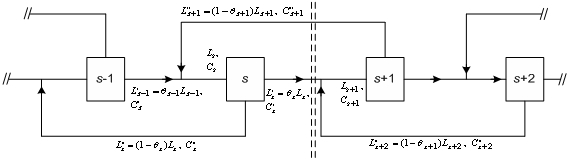
\includegraphics[scale=0.9]{img/image2.png}}
  \caption{Схема соединения ступеней в симметричном противоточном каскаде.}\label{image2}
\end{figure}

Изображенная на рис. \cite{image2}. схема характерна тем, что между любыми соседними ступенями можно провести поперечное сечение (на рисунке изображено двойной пунктирной линией), пересекающее только две коммуникации. Такой каскад называют \textit{симметричным.}

Если потоки направляют не в соседние предыдущую и последующую ступени, а через одну или через несколько ступеней, то такой противоточный каскад называется \textit{несимметричным} (рис. \cite{unsymmetr}).

\begin{figure}[ht]
  \centerfloat{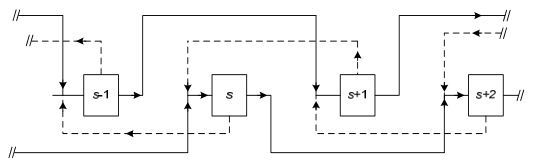
\includegraphics[scale=0.9]{img/unsymmetr.png}}
  \caption{Схема соединения ступеней в несимметричный каскад с подачей потока питания через одну ступень в прямом направлении.}\label{unsymmetr}
\end{figure}


Отметим, что при внешнем каскадировании разделительная ступень считается заданной ячейкой схемы, для которой коэффициент разделения и его зависимость от коэффициента деления потоков должны быть известны, после чего сам процесс разделения оказывается для построения каскадов несущественным. Тем самым теория построения "внешних" потоков оказывается независимой от конкретного метода разделения.

\section{Разделительная способность (мощность). Работа  разделения. Разделительный потенциал.}

В технологии разделения изотопов понятие работы разделения, разделительной мощности и разделительного потенциала имеют весьма важное значение, так как их использование позволяет не прибегая к сложным расчетам оценить необходимое число элементов в каскаде и удельные затраты на производство обогащенного продукта. Количественное определение работы разделения впервые было предложено английскими физиками Пайерлсом и Дираком. Они предположили, что должна существовать функция $\tilde{U}$, с помощью которой можно охарактеризовать «ценность» изотопной смеси как в качественном, так и в количественном отношении, и которую можно представить в виде произведения экстенсивной величины -- количества разделяемой смеси \textit{M} -- на интенсивную величину -- функцию \textit{V(c)}, зависящую только от концентрации ценного изотопа и характеризующую качество смеси

\begin{equation} \label{GrindEQ__1_13_} 
\tilde{U}=MV(C).       
\end{equation} 

Функцию \textit{V(C)}, было предложено называть \textit{разделительным потенциалом}. Необходимо иметь в виду, что функция $\tilde{U}$ ничего общего со стоимостным выражением не имеет и поэтому ее не следует смешивать с реальной ценой изотопной смеси.

Процесс разделения смеси в разделительной установке (Под разделительной установкой здесь будем понимать разделительный каскад, отдельной ячейкой которого является разделительный элемент) для любого метода разделения схематически можно представить следующим образом. До начала процесса имелось некоторое количество исходной смеси \textit{F$^{*}$}(в ед. массы) с концентрацией ценного изотопа \textit{C${}_{F}$}. С использованием введенных понятий изотопная ценность этого смеси будет определяться значением функции $\tilde{U}_{F^{*} } =F^{*} V(С_{F} )$. В результате процесса разделения получают обогащенный продукт в количестве \textit{P${}^{*}$}(в ед. массы) с концентрацией ценного изотопа \textit{C${}_{P}$} и обедненный продукт в количестве \textit{W${}^{*}$}(в ед. массы) с концентрацией \textit{C${}_{W}$}. Изотопная ценность этих продуктов будет $\tilde{U}_{P^{*} } =P^{*} V(C_{P} )$ и $\tilde{U}_{W^{*} } =W^{*} V(C_{W} )$ соответственно. В результате проведения процесса разделения функция $\tilde{U}_{F^{*} } $ изменится на величину $\Delta \tilde{U}$:

\begin{equation} \label{GrindEQ__1_14_} 
\begin{array}{l} {\Delta \tilde{U}=\tilde{U}_{P^{*} } +\tilde{U}_{W^{*} } -\tilde{U}_{F^{*} } =} \\ {=P^{*} V(C_{P} )+W^{*} V(C_{W} )-F^{*} V(C_{F} )} \end{array}           
\end{equation} 

Следовательно «ценность» смеси будет выражаться соотношением

\begin{equation}\label{GrindEQ__1_15_} 
F^{*} V(C_{F} )+\Delta \tilde{U}=P^{*} V(C_{P} )+W^{*} V(C_{W} ).      
\end{equation} 

Из соотношения \ref{GrindEQ__1_15_} следует, что величина $\Delta \tilde{U}$ характеризует меру усилий, которую необходимо затратить на получение из первоначальной бинарной смеси изотопов два новых продукта -- обогащенный и обедненный одним из изотопов этой смеси. Приращение функции $\tilde{U}$, характеризующее перераспределение первоначальной массы разделяемого вещества между двумя выходными потоками и изменение изотопного состава в них при прохождении смеси через разделительную установку, называется \textit{работой разделения}. Введенное понятие работы разделения не имеет ничего общего с реальными энергетическими затратами на поддержание внешних и внутренних потоков в разделительной установке. Из формулы \ref{GrindEQ__1_14_} следует, что введенная таким образом работа разделения имеет размерность количества вещества. 

 Отметим также, что величина работы разделения не дает ответ на вопрос о том, за какое время эта работа может быть выполнена на той или иной разделительной установке. Для получения ответа на это вопрос необходимо знать \textit{разделительную мощность (способность)} установки $\Delta U$, то есть работу разделения, выполняемую установкой в единицу времени. Для перехода от $\Delta \tilde{U}$ к $\Delta U$ достаточно в соотношении \ref{GrindEQ__1_14_} вместо $F^{*} ,P^{*} ,W^{*} $ подставить величины входящего (\textit{F}) и выходящих (\textit{P} и \textit{W}) в установку потоков соответственно.

\begin{equation} \label{GrindEQ__1_16_} 
\Delta U=PV(C_{P} )+WV(C_{W} )-FV(C_{F} ).     
\end{equation} 

Для вычисления работы разделения и разделительной способности необходимо знать явный вид функции \textit{V(C)}. Пайерлс и Дирак решили этот вопрос, рассматривая разделительную способность ступени (элемента), которую в соответствии с вышесказанным можно выразить следующим образом:

\begin{equation} \label{GrindEQ__1_17_} 
\delta U=\theta LV(C')+(1-\theta )LV(C'')-LV(C).   
\end{equation} 

В случае слабого разделения (\textit{q}$\mathrm{\sim}$1) функции $V(A')$ и $V(A'')$ можно разложить в ряд Тейлора в окрестности точки $A$, ограничиваясь членами второго порядка малости

\begin{equation} \label{GrindEQ__1_18_} 
V(A')\approx V(A)+\frac{dV}{dA} \delta '+\frac{1}{2} \frac{d^{2} V}{dA^{2}} (\delta ')^{2} ,        
\end{equation}

\begin{equation} \label{GrindEQ__1_19_} 
V(A'')\approx V(A)-\frac{dV}{dA} \delta ''+\frac{1}{2} \frac{d^{2} V}{dA^{2} } (\delta '')^{2} .     
\end{equation} 

Подставив их в \ref{GrindEQ__1_17_}, находим

\begin{equation} \label{GrindEQ__1_20_} 
\begin{array}{l} {\delta U=\left[\theta L+(1-\theta )L-L\right]{\kern 1pt} {\kern 1pt} {\kern 1pt} V(A)+\left[\theta L\delta '-(1-\theta )L\delta ''\right]\frac{dV}{dA} +} \\ {\, \, \, \, \, \, \, \, \, \, \, \, \, \, \, \, \, \, \, \, \, +\frac{1}{2} \left[\theta L(\delta ')^{2} +(1-\theta )L(\delta '')^{2} \right]\frac{d^{2} V}{dA^{2} } \, \, \, .} \end{array} 
\end{equation} 

Из условий баланса \ref{GrindEQ__1_1_}, \ref{GrindEQ__1_2_} и \ref{GrindEQ__1_12_} коэффициенты при $V(A)$ и ${dV \mathord{\left/{\vphantom{dV dA}}\right.\kern-\nulldelimiterspace} dA} $ равны нулю. Поэтому с учётом \ref{GrindEQ__1_11_} и \ref{GrindEQ__1_12_} имеем

\begin{equation} \label{GrindEQ__1_21_} 
\delta U=\frac{1}{2} \theta (1-\theta )L\varepsilon ^{2} \frac{d^{2} V}{dA^{2} } A^{2} (1-A)^{2} .           
\end{equation} 

Пайерлс и Дирак ввели условие, согласно которому разделительная способность (мощность) ступени или элемента определяется только его разделительными характеристиками $L,\; \theta ,\; \varepsilon $ и не должна зависеть от состава питающей его смеси. Это условие обосновывается следующим соображением. Если разделительная способность отдельной ячейки установки -- разделительного элемента -- не зависит от концентрации и все элементы работают в идентичных условиях, то есть с одинаковыми $L,\; \theta ,\; \varepsilon $, то суммарная разделительная способность элементов, составляющих эту установку, будет равна произведению $Z\cdot \delta U_{M;} $, где $\delta U_{M;} $ - разделительная способность одного элемента, \textit{Z} --число элементов в установке. Если процесс разделения организован так, что потери работы разделения (разделительной способности) отсутствуют, то величина $Z\cdot \delta U_{M;} $ будет равна разделительной способности всей установки $\Delta U$, вычисляемой по формуле \ref{GrindEQ__1_16_}, то есть

\begin{equation} \label{GrindEQ__1_22_} 
\Delta U=Z\cdot \delta U_{M;} .       
\end{equation} 

Откуда число разделительных элементов в каскаде будет определяться по формуле

\begin{equation} \label{GrindEQ__1_23_} 
Z=\frac{\Delta U}{\delta U_{M;} }  .        
\end{equation} 

Таким образом, если условие независимости разделительной способности от концентрации выполнено, то появляется возможность вычислить важную характеристику процесса разделения -- суммарное число элементов, обеспечивающих необходимую разделительную способность установки для решения заданной разделительной задачи.

Условие независимости разделительной способности ступени (элемента) от концентрации приводит к следующему уравнению:

\begin{equation} \label{GrindEQ__1_24_} 
\delta U=\frac{1}{2} \theta (1-\theta )L\varepsilon ^{2} \frac{d^{2} V}{dc^{2} } c^{2} (1-c)^{2} =const.   
\end{equation} 

Если в уравнении \ref{GrindEQ__1_24_} выбрать постоянную в виде

\begin{equation} \label{GrindEQ__1_25_} 
const=\frac{1}{2} \theta (1-\theta )L\varepsilon ^{2} ,     
\end{equation}

то для определения потенциала \textit{V}(\textit{c}) получается дифференциальное уравнение

\begin{equation} \label{GrindEQ__1_26_} 
\frac{d^{2} V}{dc^{2} } =\frac{1}{c^{2} (1-c^{2} )} ,      
\end{equation}

общее решение которого имеет вид:

\begin{equation} \label{GrindEQ__1_27_} 
V(c)=(2c-1)\ln \frac{c}{1-c} +ac+b.    
\end{equation} 

Произвольные постоянные в выражении \ref{GrindEQ__1_27_} должны быть определены дополнительными условиями. Однако нетрудно видеть, что эти постоянные не имеют существенного значения, так как при вычислении работы разделения по формуле \ref{GrindEQ__1_15_} или разделительной способности по формуле \ref{GrindEQ__1_16_} они не входят в окончательный результат с учетом уравнений материального баланса. Поэтому, следуя Пайерлсу, можно положить $a=b=0$ и тогда потенциал приобретает вид

\begin{equation} \label{GrindEQ__1_28_} 
V(C)=(2A-1)\ln \frac{A}{1-A}.                            
\end{equation} 

\begin{figure}[ht]
  \centerfloat{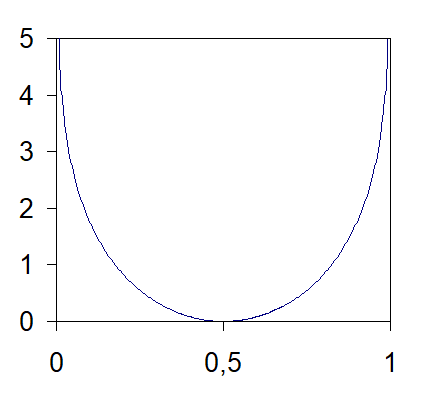
\includegraphics[scale=0.6]{img/image1}}
  \caption{Зависимость разделительного потенциала от концентрации.}\label{image1}
\end{figure}

В этой форме его обычно называют потенциалом Пайерлса-Дирака. Графический вид функции $V(A)$ показан на рис. \ref{image1}. 

Разделительный потенциал Пайерлса-Дирака и его производная равны нулю при \textit{с}=0,5. При любых других значениях концентрации потенциал \textit{V}(\textit{c})$\mathrm{>}$0, а при \textit{с}$\rightarrow$0 или \textit{с}$\rightarrow$$\propto$ потенциал \textit{V}(\textit{c}) $\rightarrow$$\propto$, что означает необходимость бесконечно большой работы разделения для получения чистых изотопных продуктов.

Таким образом, в случае «слабого обогащения» разделительный потенциал определяется формулой \ref{GrindEQ__1_28_}, а разделительная способность -- соотношением \ref{GrindEQ__1_25_}.

Какой физический смысл имеет разделительная способность? Пайерлс и Фукс установили прямую связь величины $\delta U$ с уменьшением энтропии смеси в единицу времени $\Delta S_\textup{разд.}$, которое имеет место при стационарной работе разделительной ступени (элемента). Величину $\Delta S_\textup{разд.}$ можно рассчитать из следующих соображений. Энтропия при образовании одного моля смеси идеальных газов или сильно разбавленного раствора из чистых компонентов равна 

\begin{equation} \label{GrindEQ__1_29_} 
S=-\tilde{R}\left[c\ln c+(1-c)\ln (1-c)\right],       
\end{equation} 

где $\tilde{R}$ - газовая постоянная.

Если из \textit{L} молей питающей смеси с концентрацией \textit{C} получается на выходе ступени (элемента) в единицу времени $L'=\theta L$ молей обогащенного до концентрации $C'$, и $L''=(1-\theta )L$ молей, обедненных до концентрации $C''$, то изменение энтропии в единицу времени $\Delta S_\textup{разд.}$ будет равно

\begin{equation} \label{GrindEQ__1_30_} 
\Delta S_\textup{разд.} =\mathrm{\; -}\left[LS(C)-\theta LS(C')-(1-\theta )LS(C'')\right].    
\end{equation} 

В случае «слабого разделения» выражение для $\Delta S_\textup{разд.} $ заметно упрощается, если соотношение \ref{GrindEQ__1_30_} представить в виде

\begin{equation} \label{GrindEQ__1_31_} 
\Delta S_\textup{разд.} =\theta LS(C+\delta ')+(1-\theta )LS(C-\delta '')-LS(C).   
\end{equation} 

Разлагая в ряд функции $S(C+\delta ')$ и $S(C-\delta '')$ в ряд Тейлора в окрестности точки \textit{C} и ограничиваясь членами второго порядка малости, после несложных преобразований получаем

\begin{equation} \label{GrindEQ__1_32_} 
\Delta S_\textup{разд.} =\frac{\theta (1-\theta )}{2} \delta ^{2} \frac{d^{2} S}{dc^{2} } .       
\end{equation} 

Учитывая, что $\delta =\varepsilon c(1-c)$ и $\frac{d^{2} S}{dc^{2} } =-\frac{\tilde{R}}{c(1-c)} $, и подставляя выражение \ref{GrindEQ__1_32_} в \ref{GrindEQ__1_31_}, получим

\begin{equation} \label{GrindEQ__1_33_} 
\Delta S_\textup{разд.} =-\frac{\theta (1-\theta )}{2} L\varepsilon ^{2} \tilde{R}C(1-C),      
\end{equation} 

которое с учетом выражения \ref{GrindEQ__1_25_} может быть переписано в виде

\begin{equation} \label{GrindEQ__1_34_} 
\Delta S_\textup{разд.} =-\delta U\cdot \tilde{R}C(1-C)       
\end{equation} 

Из полученного выражения \ref{GrindEQ__1_34_} следует, что величина разделительной способности $\delta U$ прямо пропорциональна уменьшению величины безразмерной энтропии смеси $\Delta S_\textup{разд.} /\tilde{R}$. Изменение концентраций компонентов в смеси газов связано с изменением меры порядка. В общем случае мерой порядка служит энтропия. В соответствии с \ref{GrindEQ__1_34_} уменьшение энтропии при разделении на ступени произведению концентраций компонентов изотопной смеси \textit{c}(1-\textit{c}). Это произведение определяет вероятность нахождения в смеси пары различных молекул. Вследствие этого разделительная способность ступени равна уменьшению безразмерной энтропии, отнесенной к величине этой вероятности. Таким образом, разделительная ступень увеличивает меру порядка в смеси изотопов. Скорость увеличения этой меры определяет разделительную способность ступени. 

Перейдем теперь к случаю, когда коэффициент разделения ступени \textit{q} заметно отличается от единицы. При произвольных значениях полного коэффициента разделения \textit{q} функциональное уравнение 
\begin{equation} \label{GrindEQ__1_35_} 
\delta U=\theta LV(C')+(1-\theta )LV(C'')-LV(C)=const 
\end{equation} 

имеет решение, при котором функция \textit{V} зависит только от концентрации в случае симметричной работы ступени, то есть когда $\alpha =\beta =\sqrt{q} $ [1].

 Если процесс разделения в ступени симметричен, то выполняются условия

 \begin{equation} \label{GrindEQ__1_36_} 
R'=\alpha R,\; \; R''=\frac{1}{\alpha } R,\; \; \theta =\frac{1+\alpha R}{(\alpha +1)(1+R)} ,\; \; 1-\theta =\frac{\alpha +R}{(\alpha +1)(1+R)} , 
\end{equation} 
где $R=\frac{C}{1-C} $.

 Подставляя \ref{GrindEQ__1_36_} в \ref{GrindEQ__1_35_}, имеем 
\begin{equation} \label{GrindEQ__1_37_} 
\frac{\delta U}{L} =\frac{1+\alpha R}{(\alpha +1)(1+R)} V(\alpha R)+\frac{\alpha (1+\frac{R}{\alpha } )}{(\alpha +1)(1+R)} V\left(\frac{R}{\alpha } \right)-V(R)=const. 
\end{equation} 

Введем новую переменную \textit{l} следующим образом:
\begin{equation} \label{GrindEQ__1_38_} 
R=R_{0} \alpha ^{l} ,       
\end{equation} 

где \textit{R}${}_{0}$ -- константа, и положим, что
\begin{equation} \label{GrindEQ__1_39_} 
(1+R)V(R)\equiv F(l).     
\end{equation} 

С учетом \ref{GrindEQ__1_38_} и \ref{GrindEQ__1_39_} уравнение \ref{GrindEQ__1_37_} трансформируется в классическое разностное уравнение второго порядка
\begin{equation} \label{GrindEQ__1_40_} 
F(l+1)+\alpha F(l-1)-(\alpha +1)F(l)=A(\alpha +1)(1+R_{0} \alpha ^{l} ),   
\end{equation} 

где \textit{A} -- константа.

Общее решение уравнения \ref{GrindEQ__1_40_} можно представить в виде
\begin{equation} \label{GrindEQ__1_41_} 
F(l)=A\frac{\alpha +1}{\alpha -1} l(R_{0} \alpha ^{l} -1)+a\alpha ^{l} +b),    
\end{equation} 

где \textit{a }и \textit{b} также константы.

Используя выражения \ref{GrindEQ__1_37_} и \ref{GrindEQ__1_41_}, найдем вид функции \textit{V}(\textit{R)}
\begin{equation} \label{GrindEQ__1_42_} 
V(R)=A\frac{\alpha +1}{(\alpha -1)\ln \alpha } \left[(2c-1)\ln \frac{R}{R_{0} } +a\ln \alpha \frac{c}{R} +b\ln \alpha (1-c)\right].  
\end{equation} 

Выбирая константу \textit{A} равной $A=\frac{\delta U}{L} =\frac{\alpha -1}{\alpha +1} \ln \alpha $ и полагая, что $R_{0} =1,\quad a=0,\quad b=0$${}^{*}$ (Как и в случае «слабого обогащения», эти константы не входят в окончательные выражения для разделительного потенциала и разделительной способности), получим для разделительного потенциала и разделительной способности следующие выражения:

\begin{equation} \label{GrindEQ__1_43_} 
V(c)=(2c-1)\ln \frac{c}{1-c} ,        
\end{equation} 

\begin{equation} \label{GrindEQ__1_44_} 
\delta U=L\frac{(\alpha -1)\ln \alpha }{\alpha +1} \equiv L\frac{\left(\sqrt{q} -1\right)\ln \sqrt{q} }{\sqrt{q-1} } .     
\end{equation} 

Очевидно, что в случае «слабого разделения» $(\varepsilon =q-1<<1)$ формула \ref{GrindEQ__1_44_} переходит в формулу \ref{GrindEQ__1_25_} при $\theta =1/2$. Отметим, что соотношения \ref{GrindEQ__1_25_}, \ref{GrindEQ__1_28_} и \ref{GrindEQ__1_44_}, полученные на основе подхода Пайерлса-Дирака, полностью подтверждаются результатами теории идеальных каскадов из симметричных ступеней, разработанной К.Коэном.

В случае несимметричной работы ступени $(\alpha \ne \beta )$ при произвольном обогащении на ступени выполнить оба условия Пайерлса-Дирака, а именно

- разделительный потенциал зависит только от изотопного состава смеси;

- разделительная способность ступени определяется только характеристиками самой ступени;

не удается. Разделительная способность ступени зависит от коэффициентов разделения $(\alpha ,\beta)$ и концентрации смеси. Как будет показано ниже, при больших $(1-c<<1)$ и малых $(c<<1)$ концентрациях величина $\delta U$ от концентрации не зависит. Разделительный потенциал, полученный из решения функционального уравнения \ref{GrindEQ__1_35_} оказывается зависящим не только от состава смеси, но и коэффициентов разделения ступени, то есть $V(c,\alpha ,\beta)$.

На основе разделительного потенциала, записанного в виде \ref{GrindEQ__1_28_}, введены единицы работы разделения изотопов урана. В настоящее время его используют и в случае произвольных коэффициентов разделения на ступени, работающей в несимметричном режиме [38, 52]. Теоретическое обоснование подобного подхода, проведенного в различных работах, связано, в частности, с изменением условий Пайерлса-Дирака \cite{baranovIzotopySvoystvaPoluchenie} и рассмотрением идеализированного процесса разделения \cite{yamamotoMulticomponentIsotopeSeparating1978}.

Исходя из общего соотношения для разделительной способности ступени
\begin{equation} \label{GrindEQ__1_45_} 
\delta U=\theta LV(c')+(1-\theta )LV(c'')-LV(c) 
\end{equation} 

и разделительного потенциала, определяемого по формуле \ref{GrindEQ__1_28_}, можно найти формулу при всех значениях $q$ и $(\alpha \ne \beta )$ [8, 9]. Поскольку $A=\frac{R}{R+1} ,\; \; 2A-1=\frac{R-1}{R+1} $, разделительный потенциал \ref{GrindEQ__1_28_} может быть представлен в виде

\begin{equation} \label{GrindEQ__1_46_} 
V^{*} (R)=\frac{R-1}{R+1} \ln R,                            
\end{equation} 

где индекс «звездочка» означает то, что разделительный потенциал рассматривается как функция новой переменной $R$.

Соотношение для определения разделительной способности ступени запишется в виде

\begin{equation} \label{GrindEQ__1_47_} 
\delta U=L[\theta V^{*} (R')+(1-\theta )V^{*} (R'')-V(R)].    
\end{equation} 

Формулу для определения коэффициента деления потока нетрудно получить, комбинируя выражения \ref{GrindEQ__1_3_}, \ref{GrindEQ__1_7_} и \ref{GrindEQ__1_9_}:

\begin{equation} \label{GrindEQ__1_48_} 
\theta =\frac{\left(\beta -1\right)\left[1+(\alpha -1)c\right]}{\alpha \beta -1} .        
\end{equation} 

Замена в \ref{GrindEQ__1_48_} концентрации \textit{с} на отношение $R/(1-R)$ приводит к выражениям

\begin{equation} \label{GrindEQ__1_49_} 
\theta =\frac{\left(\alpha R+1\right)\mathrm{\; }\left(\beta -1\right)}{\left(R+1\right)\mathrm{\; }\left(\alpha \beta -1\right)} ,         
\end{equation} 
\begin{equation} \label{GrindEQ__1_50_} 
1-\theta =\frac{\left(R+\beta \right)\mathrm{\; }\left(\alpha -1\right)}{\left(R+1\right)\mathrm{\; }\left(\alpha \beta -1\right)} .         
\end{equation} 

Подставляя \ref{GrindEQ__1_46_}, \ref{GrindEQ__1_49_} и \ref{GrindEQ__1_50_} в \ref{GrindEQ__1_47_} с учетом $R'=\alpha R,\; R''=\frac{1}{\beta } R$ и $\alpha \beta =q$, получим

\begin{equation} \label{GrindEQ__1_51_} 
\begin{array}{l} {\delta U=L\frac{1}{q-1} \left\{\left[\left(\alpha -1\right)\beta \ln \beta -\left(\beta -1\right)\ln \alpha \right]\frac{1}{R+1} +\right. } \\ {\left. +\left[\left(\beta -1\right)\alpha \ln \alpha -\left(\alpha -1\right)\ln \beta \right]\frac{R}{R+1} \right\}} \end{array}.  
\end{equation} 

Переходя в \ref{GrindEQ__1_51_} от относительных концентраций \textit{R} к абсолютным, окончательно получим

\begin{equation} \label{GrindEQ__1_52_} 
\delta U=L[f_{1} (\alpha ,\beta )(1-A)+f_{2} (\alpha ,\beta )A], 
\end{equation} 

где
\begin{equation} \label{GrindEQ__1_53_} 
  f_{1} (\alpha ,\beta )=\frac{(\alpha -1)\beta \ln \beta -(\beta -1)\ln \alpha }{\alpha \beta -1} ,  
\end{equation} 

\begin{equation} \label{GrindEQ__1_54_} 
f_{2} (\alpha ,\beta )=\frac{(\beta -1)\alpha \ln \alpha -(\alpha -1)\ln \beta }{\alpha \beta -1} ,  
\end{equation} 

Из \ref{GrindEQ__1_52_} следует, что разделительная способность ступени $\delta U$ в общем случае является функцией концентрации. Зависимость от концентрации исчезает в следующих частных случаях.

1. Случай слабого разделения, $\alpha -1<<1,\; \; \beta -1<<1$. Так как в этом случае $\alpha $~и~$\beta $ близки к единице, то

\begin{equation} \label{GrindEQ__1_55_} 
\ln \alpha \approx (\alpha -1)-\frac{1}{2} (\alpha -1)^{2} +\cdot \cdot \cdot , 
\end{equation} 

\begin{equation} \label{GrindEQ__1_56_} 
\ln \beta \approx (\beta -1)-\frac{1}{2} (\beta -1)^{2} +\cdot \cdot \cdot , 
\end{equation} 

Имея в виду \ref{GrindEQ__1_7_}, \ref{GrindEQ__1_11_} и \ref{GrindEQ__1_12_}, подставляя \ref{GrindEQ__1_55_} и \ref{GrindEQ__1_56_} в \ref{GrindEQ__1_52_} и сохраняя малые величины 2-ого порядка, имеем
\begin{equation} \label{GrindEQ__1_57_} 
\delta U=\frac{L}{2} (\alpha -1)(\beta -1)\approx \frac{L}{2} \varepsilon '\varepsilon ''=\frac{\theta (1-\theta )L\varepsilon ^{2} }{2} ,             
\end{equation} 

что соответствует классическому виду для разделительной способности \ref{GrindEQ__1_25_}.

2. Случай симметричной ступени при произвольном на ней обогащении. При $\alpha =\beta $ \ref{GrindEQ__1_52_} преобразуется к виду
\begin{equation} \label{GrindEQ__1_58_} 
\delta U=L\frac{(\alpha -1)\alpha \ln \alpha -(\alpha -1)\ln \alpha }{\alpha ^{2} -1} =L\frac{(\alpha -1)\ln \alpha }{\alpha +1} ,              
\end{equation} 

что также соответствует классической формуле \ref{GrindEQ__1_44_}.

3. Случай малых концентраций, $A<<1.$ При $A<<1,\; \; 1-A\approx 1$ выражение \ref{GrindEQ__1_52_} преобразуется к виду
\begin{equation} \label{GrindEQ__1_59_} 
\delta U=Lf_{1} (\alpha ,\beta )=L\frac{(\alpha -1)\beta \ln \beta -(\beta -1)\ln \alpha }{\alpha \beta -1} .                     
\end{equation} 

В рассматриваемом случае выражение \ref{GrindEQ__1_49_} упрощается
\begin{equation} \label{GrindEQ__1_60_} 
\theta =\frac{\beta -1}{\alpha \beta -1} .                                        
\end{equation} 

Соответственно, величина $\beta $ равна
\begin{equation} \label{GrindEQ__1_61_} 
\beta =1+\theta (\alpha \beta -1).                            
\end{equation} 

Учёт \ref{GrindEQ__1_60_} и \ref{GrindEQ__1_61_} и связи$\alpha \beta =q$ позволяет преобразовать соотношение \ref{GrindEQ__1_59_} к виду
\begin{equation} \label{GrindEQ__1_62_} 
\delta U=L\{ \ln [1+\theta (q-1)]-\theta \ln q\} .            
\end{equation} 

Это выражение для разделительной способности имеет важное значение при расчетах каскадов для получения слабообогащенного урана. 

4. В случае больших концентраций, когда выполняется $(c\approx 1)$ выражение \ref{GrindEQ__1_42_} преобразуется к виду
\begin{equation} \label{GrindEQ__1_63_} 
\delta U=Lf_{2} (\alpha ,\, \beta )=L\frac{\beta (\alpha -1)\ln \beta -(\beta -1)\ln \alpha }{q-1} .     
\end{equation} 

В этом случае коэффициент деления потока запишется как
\begin{equation} \label{GrindEQ__1_64_} 
\theta =\frac{q(\beta -1)}{\beta (q-1)} ,         
\end{equation} 

а выражение для разделительной способности с учётом соотношения $q=\alpha \beta $ будет иметь вид
\begin{equation} \label{GrindEQ__1_65_} 
\delta U=L\left\{\ln \left[q-\theta (q-1)\right]-(1-\theta )\ln q\right\}.      
\end{equation} 

Коэффициент разделения по обеднённой фракции $\beta $ в формуле для разделительной способности \ref{GrindEQ__1_52_} можно выразить через $\alpha $. Тогда после дифференцирования удельной разделительной способности $\delta U/L$ по $\alpha $ и приравнивания производной нулю, получим квадратное уравнение относительно $\alpha $ [10, 22]:

\begin{equation} \label{GrindEQ__1_66_} 
a\alpha ^{2} -b\alpha -d=0,          
\end{equation} 

в котором $a=c\frac{\ln q}{q-1} ,\quad b=2c-1,\quad d=(1-c)\frac{\ln q}{q-1} \mathrm{\; }q\; .$

Квадратное уравнение \ref{GrindEQ__1_66_} имеет только одно физическое решение, обеспечивающее максимум величины $\delta U/L$:
\begin{equation} \label{GrindEQ__1_67_} 
\alpha_\textup{опт.} =\frac{q}{\beta_\textup{опт.}} =\frac{b+\sqrt{b^{2} +4ad} }{2} .      
\end{equation} 

Нетрудно видеть, что, во-первых, решение \ref{GrindEQ__1_67_} зависит от величин $q$ и $C$, а, во-вторых, независимо от величины $q$ при $C=0,5$ максимальное значение $\alpha_\textup{опт.} $ будет равно $\alpha_\textup{опт.} =\sqrt{q}$. Следовательно, максимум удельной разделительной способности ступени при значении концентрации $C=0,5$ достигается в соответствии \ref{GrindEQ__1_67_} при симметричном режиме работы ступени, то есть при условии $\alpha $=$\beta $. При концентрациях, отличных от 0,5, максимум удельной разделительной способности не соответствует симметричному режиму работы разделительной ступени. Для интересного для практики случая $C<<1$ (получение слабообогащённого урана) отыскание максимума функции приводит к следующим значениям [11]

\begin{equation} \label{GrindEQ__1_68_} 
\theta_\textup{опт.} =\frac{1}{\ln q} -\frac{1}{q-1} ,        
\end{equation} 
\begin{equation} \label{GrindEQ__1_69_} 
\alpha_\textup{опт.} =\frac{q}{\beta_\textup{опт.}} =\frac{q\ln q}{q-1} ,        
\end{equation} 
\begin{equation} \label{GrindEQ__1_70_} 
\left(\frac{\delta U}{L} \right)_{\max } =\ln \left[\frac{(q-1)}{\ln q} \right]+\frac{\ln q}{q-1} -1.    
\end{equation} 

Отметим, что выражение \ref{GrindEQ__1_69_} для $\alpha_\textup{опт.} $ может быть получено из \ref{GrindEQ__1_67_} подстановкой условия $C<<1$.

% В таблице 1.1 приведены величины $\theta ,\; \alpha ,\; \beta \; $ и $\delta U/L$ разделительной ступени для симметричного случая $(\alpha =\beta )$ и случая, когда ступень работает с оптимальной величиной $\theta $ в зависимости от величины \textit{q} при малых концентрациях ценного компонента (\textit{с}$\mathrm{<}$$\mathrm{<}$1).

% Таблица 1.1.

% \noindent Характеристики разделительной ступени каскада при симметричном и оптимальном разделении для различных значений \textit{q} и \textit{с}$\mathrm{<}$$\mathrm{<}$1

% \begin{tabular}{|p{0.7in}|p{0.5in}|p{0.4in}|p{0.4in}|p{0.4in}|p{0.5in}|} \hline 
% \textit{q} & 1,1 & 1,6 & 3,0 & 5,0 & 10,0 \\ \hline 
% \textit{$\theta$}${}_{\textrm{с}\textrm{и}\textrm{м}}$ & 0,488 & 0441 & 0,366 & 0,309 & 0,240 \\ \hline 
% \textit{$\theta$}${}_{\textrm{о}\textrm{п}\textrm{т}}$ & 0,492 & 0,461 & 0,401 & 0,371 & 0,323 \\ \hline 
% \textit{$\alpha$}${}_{\textrm{с}\textrm{и}\textrm{м}}$ & 1,0488 & 1,2649 & 1,7320 & 2,2361 & 3,1623 \\ \hline 
% \textit{$\alpha$}${}_{\textrm{о}\textrm{п}\textrm{т}}$ & 1,0484 & 1,2532 & 1,6780 & 2,0118 & 2,5584 \\ \hline 
% \textit{$\beta$}${}_{\textrm{с}\textrm{и}\textrm{м}}$ & 1,0488 & 1,2649 & 1,7320 & 2,2361 & 3,1623 \\ \hline 
% \textit{$\beta$}${}_{\textrm{о}\textrm{п}\textrm{т}}$ & 1,0492 & 1,2766 & 1,8204 & 2,4853 & 3,9087 \\ \hline 
% $\left(\delta U/L\right)$${}_{\textrm{с}\textrm{и}\textrm{м}}$ & 1,134$.$10${}^{-3}$ & 0,0275 & 0,1471 & 0,3075 & 0,5980 \\ \hline 
% $\left(\delta U/L\right)$${}_{\textrm{м}\textrm{а}\textrm{к}\textrm{с}}$ & 1,135$.$10${}^{-3}$ & 0,0276 & 0,1483 & 0,3128 & 0,6190 \\ \hline 
% $\frac{\left(\delta U/L\right)_{<0:A} -\left(\delta U/L\right)_{A8<} }{\left(\delta U/L\right)_{A8<} } $,\% & 0,088 & 0,364 & 0,817\newline  & 1,723 & 3,512 \\ \hline 
% \end{tabular}

% Видно, что с возрастанием \textit{q} увеличивается разница между максимально возможным значением $\left(\delta U/L\right)$${}_{\textrm{м}\textrm{а}\textrm{к}\textrm{с}}$, получаемым при $\alpha \ne \beta $, и $\left(\delta U/L\right)$${}_{\textrm{с}\textrm{и}\textrm{м}}$, соответствующим симметричному разделению в ступени.

% Как будет показано в разделе 1.8 рассмотренные особенности разделения существенны для анализа эффективности работы многоступенчатых установок.

\section{Получение уравнений симметрично-противоточного каскада для случая произвольного числа компонентов и произвольных коэффициентов разделения.}

Рассмотрим симметричный каскад, состоящий из \textit{N} ступеней. 

Пусть на вход ступени с номером $s=f$ подают поток питания $F$ с концентрацией $A_{F} $. Поток, обогащенный ценным (целевым) изотопом, отбирается с правого конца каскада $(s=N)$ (сокращенно: отбор), а обедненный поток - с левого конца каскада $(s=1)$ (сокращенно: отвал). Соответственно обозначим концентрации в потоках отбора $A_{P} $ и отвала $A_{W} $. Ступени каскада нумеруются последовательно от 1 на отвале до \textit{N} на отборе. Часть каскада от точки подачи питания $(s=f,\; \; f+1,\; { ...}\; {,}\; \; {N)}$ называется обогатительной, а часть слева $(s=1,\; \; 2,\; \; {...}\; {,}\; \; f{ -1)}$ - обеднительной.

В симметричной противоточной схеме можно использовать частичный или полный возврат обогащённых или обеднённых потоков отбора или отвала на вход соответствующей ступени $(s=N$ или $s=1)$. Такие коммутации потоков называют "закрутками" и обычно их применяют на концевых ступенях каскада [5] (рис. \ref{loop}).

\begin{figure}[ht]
  \centerfloat{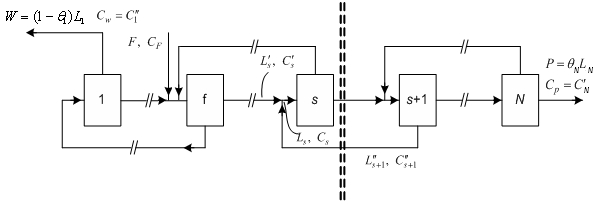
\includegraphics[scale=0.6]{img/image3.png}}
  \caption{Схема симметричного каскада для разделения бинарных смесей.}\label{loop}
\end{figure}

\begin{figure}[ht]
  \centerfloat{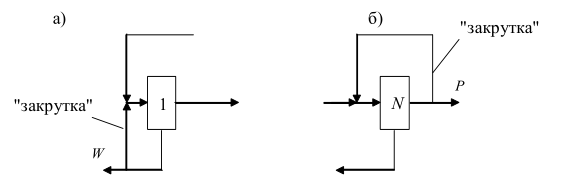
\includegraphics[scale=0.99]{img/loop.png}}
  \caption{Схемы закруток потоков : а) -- на отвале; б) -- на отборе.}\label{loop}
\end{figure}


Внешними параметрами каскада являются шесть переменных, определяющих внешние рабочие условия: $F,\; P,\; W$ - потоки питания, отбора и отвала каскада; $A_{F} ,\; A_{P} ,\; A_{W}$ - концентрации в соответствующих потоках. К внутренним относятся: \textit{N} -- общее количество ступеней в каскаде, \textit{f} -- номер ступени, на вход которой подают поток питания, параметры ступеней: $L_{S} ,\; L'_{S} ,\; L''_{S} $ - входной и два выходных потока на s-ой ступени каскада, $A_{S} ,\; A'_{S} ,\; A''_{S} \; $- концентрации в соответствующих потоках; $q_{S} ,\; \alpha _{S} ,\; \beta _{S} $ - коэффициенты разделения и $\theta _{S} $ - коэффициенты деления потоков $(s=\overline{1,N)}$.

В стационарном состоянии каскада внутренние параметры каскада можно выразить через внешние параметры каскада и уравнения разделения в ступени. Проведем поперечное сечение между некоторой \textit{s} -- ой ступенью и соседней с ней \textit{s}+1 -- ой ступенью обогатительной части каскада (обозначено на рис. \ref*{loop} пунктиром) и рассмотрим часть каскада, находящуюся справа от этого мысленного сечения. Потоки разделяемого вещества и потоки ценного (целевого) изотопа входящие в эту часть каскада $L'_{S} =\theta _{S} L_{S} $ и $L'_{S} A'_{S} =\theta _{S} L_{S} A_{s}^{/} $ и выходящие из нее $L''_{S+1} =(1-\theta _{S+1} )L_{S+1} $ и $L''_{S+1} A''_{S+1} =(1-\theta _{S+1} )L_{S+1} A''_{S+1} $ связаны уравнениями материального баланса:

\begin{equation} \label{GrindEQ__1_71_} 
\theta _{S} L_{S} -(1-\theta _{S+1} )L_{S+1} =P,                
\end{equation} 

\begin{equation} \label{GrindEQ__1_72_} 
\theta _{S} L_{S} C'_{S} -(1-\theta _{S+1} )L_{S+1} C''_{S+1} =PC_{P}.     
\end{equation} 

В этих уравнениях через, $C'_{s}$ и $C''_{s}$ обозначены концентрации ценного (целевого) изотопа соответственно на выходах из ступени.

Аналогичные соотношения можно записать для обеднительной части каскада

\begin{equation} \label{GrindEQ__1_73_} 
  \theta _{s} L_{s} -(1-\theta _{s+1} )L_{s+1} =-W, 
\end{equation}

\begin{equation} \label{GrindEQ__1_74_} 
  \theta _{s} L_{s} c'_{s} -(1-\theta _{s+1})L_{s+1} c''_{s+1} =-WC_{w}. 
\end{equation} 

Для ступени с номером \textit{s=f}, на вход которой подают поток питания \textit{F}, уравнения материального баланса имеют вид
\begin{equation} \label{GrindEQ__1_75_} 
L_{f} =\theta _{f-1} L_{f-1} +(1-\theta _{f+1} )L_{f+1} +F,     
\end{equation}

\begin{equation} \label{GrindEQ__1_76_}
  L_{f} c_{f} = \theta _{f-1} L_{f-1} c'_{f-1} + (1-\theta _{f+1})L_{f+1} c''_{f+1} +Fc_{F}.  
\end{equation}

При использовании формул \ref{GrindEQ__1_71_} -- \ref{GrindEQ__1_74_} следует иметь в виду, что $L_{0} =0$ и $L_{N+1} =0$. Концентрации $c_{S} ,\; c'_{S} $ и $c''_{S} $ на каждой ступени связаны соотношениями \ref{GrindEQ__1_4_}, \ref{GrindEQ__1_6_}, \ref{GrindEQ__1_7_}, а внешние параметры при отсутствии потерь вещества в ступенях каскада должны удовлетворять уравнениям материального баланса:
\begin{equation} \label{GrindEQ__1_77_} 
F=P+W,                                       
\end{equation} 
\begin{equation} \label{GrindEQ__1_78_} 
Fc_{F} {}^{} =Pc_{P} {}^{} +Wc_{W} {}^{} .                      
\end{equation} 

Вводя для разности концентраций на входах двух произвольных соседних  ступеней обозначение

\begin{equation} \label{GrindEQ__1_79_} 
\Delta _{S} =c_{S+1} -c_{S} ,\; (s=1,N-1) 
\end{equation} 

и, вычитая соотношение \ref{GrindEQ__1_71_}, умноженное на $c_{S} $, из \ref{GrindEQ__1_72_}, получим

\begin{equation} \label{GrindEQ__1_80_} 
\Delta _{S} =\frac{\theta _{S} L_{S} }{(1-\theta _{S+1} )L_{S+1} } \delta '_{S} +\delta ''_{S+1} -\frac{P(c_{P} -c_{S} )}{(1-\theta _{S+1} )L_{S+1} } ,            
\end{equation} 

где величины $\delta '_{S} =c'_{S} -c_{S} $ и$\delta ''_{S} =c_{S} -c''_{S} $ определяются соотношениями \ref{GrindEQ__1_9_}, \ref{GrindEQ__1_7_}. Для обеднительной части каскада справедливы точно такие же уравнения, только в правой части вместо \textit{P} и $Pc_{P} $ следует подставлять --\textit{W} и $-Wc_{W} $, т.е.
\begin{equation} \label{GrindEQ__1_81_} 
\Delta _{S} =\frac{\theta _{S} L_{S} }{(1-\theta _{S+1} )L_{S+1} } \delta '_{S} +\delta ''_{S+1} -\frac{W(c_{S} -c_{W} )}{(1-\theta _{S+1} )L_{S+1} }  
\end{equation} 

С помощью уравнений \ref{GrindEQ__1_71_} -- \ref{GrindEQ__1_78_} можно рассчитать распределения концентраций и коэффициентов деления потоков по ступеням каскада, если известны коэффициенты разделения $q_{S} ,\; \alpha _{S} ,\; \beta _{S} $ и полное число ступеней в каскаде \textit{N}, номер ступени\textit{ f}, в которую вводится поток питания, и зависимость потока $L_{S} $ от номера ступени. Подобного рода задачи обычно решают численными методами с применением ЭВМ.

В случае «слабого обогащения», когда величина обогащения мала по сравнению с концентрацией во входящем в ступень потоке, т.е. $\delta _{S} /c_{S} <<1$ система уравнений, определяющих каскад \ref{GrindEQ__1_73_} -- \ref{GrindEQ__1_76_} или \ref{GrindEQ__1_80_} -- \ref{GrindEQ__1_81_} может быть подвергнута значительным упрощениям.

Если обогащение на ступени мало, то для получения на каскаде требуемых изменений концентраций, как правило, нужно большое число ступеней $(N>>1)$, т.е. каскад должен быть "длинным". В этом случае можно считать, что все параметры каскада от ступени к ступени изменяются незначительно, а величина потока изотопной смеси, проходящего через произвольную ступень, намного превосходит величину потока отбора, т.е. $L_{S} \approx L_{S+1} $, $\delta '_{S} \approx \delta '_{S+1} $, $\delta ''_{S} \approx \delta ''_{S+1} $, $\vartheta _{S} \approx \vartheta _{S+1} $ и $P/L_{S} <<1.$ Так как число ступеней в каскаде велико, а изменение параметров при переходе от ступени к ступени мало, то можно представить \textit{s} как непрерывно меняющуюся переменную, а параметры каскада $L,\; \theta ,$ и \textit{N} непрерывными функциями от этой переменной.

С учетом сказанного из уравнения баланса \ref{GrindEQ__1_71_} следует $\theta _{S} \approx 1-\theta _{S} $, т.е.
\begin{equation} \label{GrindEQ__1_82_} 
\theta _{S} \cong \frac{1}{2}  
\end{equation} 

Условие \ref{GrindEQ__1_82_} выражает основное свойство симметричного каскада с малым обогащением на отдельной ступени. Потоки в ступенях этого каскада делятся почти пополам. Полагая в \ref{GrindEQ__1_80_} $\theta _{S} \approx \frac{1}{2} $, $L_{S} \approx L_{S+1} $, $\delta '_{S} \approx \delta '_{S+1} $, $\delta ''_{S} \approx \delta ''_{S+1} $ и учитывая, что согласно \ref{GrindEQ__1_8_}, \ref{GrindEQ__1_10_} -- \ref{GrindEQ__1_12_}

\begin{equation} \label{GrindEQ__1_83_} 
\delta '_{S} =\delta ''_{S} =\frac{1}{2} \mathrm{\; }\varepsilon c_{S} (1-c_{S} ),                    
\end{equation} 

получим
\begin{equation} \label{GrindEQ__1_84_} 
\Delta _{S} =\varepsilon c_{S} (1-c_{S} )-\frac{P(c_{P} -c_{S} )}{\frac{1}{2} L_{S+1} }  
\end{equation} 

Считая параметры каскада непрерывными функциями от переменной \textit{s} и заменяя $\Delta _{S} $ на $\frac{dc}{ds} $, перепишем предыдущее соотношение в виде
\begin{equation} \label{GrindEQ__1_85_} 
\frac{dc}{ds} =\varepsilon c(1-c)-\frac{2P(c_{P} -c)}{L} ,                    
\end{equation} 

в которых $c=c(s)$ и $L=L(s)$ - соответственно распределение концентраций и потоков вдоль каскада. 

Соответствующее уравнение для обеднительной части каскада будет иметь вид
\begin{equation} \label{GrindEQ__1_86_} 
\frac{dc}{ds} =\varepsilon c(1-c)-\frac{2W(c-c_{W} )}{L} .                     
\end{equation} 

При этом потоки отбора, отвала и питания и концентрации в этих потоках по-прежнему связаны двумя уравнениями баланса \ref{GrindEQ__1_77_} и \ref{GrindEQ__1_78_}. Минимальный поток питания для каждой ступени, соответствующий данному отбору \textit{P} и концентрации $c_{P} $, можно найти из условия равенства нулю градиента концентрации \ref{GrindEQ__1_85_}, т.е.

\begin{equation} \label{GrindEQ__1_87_} 
\left(\frac{\varepsilon L}{2P} \right)_{\min } =\frac{c_{P} -c}{c(1-c)} .                                   
\end{equation} 

Уравнение \ref{GrindEQ__1_85_} можно рассматривать как частный случай общего уравнения \ref{GrindEQ__1_80_} для приращения концентраций в применении к случаю слабого обогащения. Решение задачи в этом случае гораздо проще, потому что вместо уравнения \ref{GrindEQ__1_80_} в конечных разностях мы имеем обыкновенное дифференциальное уравнение первого порядка и еще потому, что для нахождения распределения концентраций в каскаде с заданным распределением потоков $L_{S} $ достаточно проинтегрировать только одно уравнение.

Наибольшие изменения концентраций при переходе от одной ступени к другой имеют место в безотборном режиме, когда $P=W=F=0$. Такой режим можно организовать в заполненном разделяемой смесью каскаде при наличии "закруток" на концевых ступенях. Поскольку в этом случае $c''_{S} =c'_{S-1} $, то
\begin{equation} \label{GrindEQ__1_88_} 
R'_{1} =q_{1} R''_{1} ,    
\end{equation}

\begin{equation} \label{GrindEQ__1_89_} 
R'_{S} =q_{S} R''_{S} ,    
\end{equation} 

и степень разделения в каскаде $Q=R'_{N}/R''_{1}$ достигает максимальной величины

\begin{equation} \label{GrindEQ__1_90_} 
Q=\prod _{S=1}^{N}q_{S},                      
\end{equation} 

где $R'_{N} $ и $R''_{{1}} $ - относительные концентрации ценного (целевого) изотопа на концах каскада. Если все ступени в каскаде имеют одинаковые полные коэффициенты разделения, т.е. $q_{S} \equiv q$, то соотношение \ref{GrindEQ__1_90_} может быть преобразовано к виду
\begin{equation} \label{GrindEQ__1_91_} 
N=\ln Q/\ln q,     
\end{equation} 

известному как формула Фенске [12]. Она определяет минимально возможное число ступеней, необходимое для достижения заданного значения степени разделения каскада. Характерно, что число ступеней в каскаде \textit{N} не зависит от формы каскада, т.е. конкретного распределения $L_{S} $.

В случае слабых одинаковых обогащений на ступенях из \ref{GrindEQ__1_85_} и \ref{GrindEQ__1_86_} для безотборного режима каскада имеем

\begin{equation} \label{GrindEQ__1_92_} 
\frac{dc}{ds} =\varepsilon c(1-c),    
\end{equation} 

откуда после интегрирования получаем экспоненциальный закон изменения концентраций по ступеням

\begin{equation} \label{GrindEQ__1_93_} 
R_{2} =R_{1} \exp (\varepsilon s_{12} ),   
\end{equation} 

здесь $R_{1} ,\; R_{2} $ - относительные концентрации ступеней, работающих на участке каскада, определяемом концентрациями \textit{c}${}_{1}$ и \textit{c}${}_{2}$; \textit{s}${}_{12}$ -- соответствующее количество ступеней. В режимах работы каскада с непрерывным отбором и отвалом $(P\ne 0,\; W\ne 0)$ изменения концентраций на ступенях, а, следовательно, и степень разделения каскада будут меньше.

\textbf{Критерии эффективности работы каскада}

В задачах проектирования каскадов целесообразно определять их параметры, исходя из принятого критерия эффективности. Возможны два принципиальных подхода к выбору критериев.

Первый подход предполагает, что параметры ступеней могут быть выбраны из физических соображений, не связанных непосредственно с поставленной целью разделения. Физический критерий эффективности выражается требованием, чтобы энтропия при соединении потоков на входе каждой ступени не возрастала, т.е. чтобы термодинамическая работа, связанная с изменением концентрации при разделении смеси, не терялась. Для этого необходимо, чтобы концентрации различных потоков на входе в каждую ступень были одинаковыми. Для каскада с тремя внешними потоками, это соответствует выполнению условий

\begin{equation} \label{GrindEQ__1_94_} 
\begin{array}{l} {c'_{S-1} =c_{S} =c''_{S+1} ,} \\ {\; \; \; \; \; \; \; \; c_{f} =c_{F} ,} \end{array} 
\end{equation} 

или

\begin{equation} \label{GrindEQ__1_95_} 
\begin{array}{l} {R'_{S-1} =R_{S} =R''_{S+1} ,} \\ {\; \; \; \; \; \; \; \; R_{f} =R_{F} .} \end{array}
\end{equation} 

Соотношения \ref{GrindEQ__1_94_}, \ref{GrindEQ__1_95_} называются условиями несмешивания, а каскад, удовлетворяющий этим требованиям -- \textit{идеальным}. 

В другом подходе определяют практические потребности изотопного производства. Создание крупного разделительного предприятия (завода) связано с минимизацией удельных материальных затрат на производство обогащенного продукта. Эта задача весьма сложная в силу того, что необходимо определить большое число параметров, влияющих на затраты производства. Задачу оптимизации каскада можно упростить, учитывая специфику метода разделения. В общем случае задача оптимизации может быть записана в виде
\begin{equation} \label{GrindEQ__1_96_} 
\psi =\psi (u_{1} ,u_{2} ,...,u_{k} )\to \min (\max ), 
\end{equation} 

где $\Psi $ - целевая функция (показатель эффективности); $u_{1} ,\, u_{2} ,\, ...,\, u_{k} $ - независимые параметры каскада; $\min (\max )$- значение целевой функции (минимум или максимум) при оптимальных значениях независимых параметров. При использовании молекулярно-кинетических методов разделения удельные затраты на производство обогащённого продукта, как правило, пропорциональны суммарному количеству элементов в каскаде. В соответствии с этим при заданных внешних параметрах в качестве критерия оптимизации можно принять минимум суммарного количества разделительных элементов:
\begin{equation} \label{GrindEQ__1_97_} 
\Psi =\sum _{s=1}^{N}Z_{S}  \to \min , 
\end{equation} 

где \textit{Z${}_{S}$} -- число разделительных элементов в \textit{s} -- ой ступени каскада. Величина $\sum _{s=1}^{N}Z_{S}  $ при работе элементов с заданными одинаковыми потоками \textit{L${}_{\textrm{Э}}$} может быть представлена в виде

\begin{equation} \label{GrindEQ__1_98_} 
\sum _{s=1}^{n}Z_{S} =\frac{\sum _{s=1}^{N}L_{S}  }{L_{-} }  .    
\end{equation} 

и, следовательно, в этом случае целью оптимизации является минимизация суммарного потока питания ступеней

\begin{equation} \label{GrindEQ__1_99_} 
\psi =\sum _{s=1}^{N}L_{S}  \to \min .    
\end{equation} 

Данный критерий предусматривает, что все внешние параметры каскада варьируются в допустимой области их изменения до получения минимального суммарного потока. Каскад, отвечающий требованию \ref{GrindEQ__1_99_} будем называть \textit{оптимальным.}







